\documentclass[a4paper,10pt]{article}

\usepackage{multicol}
\usepackage{caption}
\usepackage[utf8]{inputenc}
\usepackage{hyperref}
\usepackage[left=2cm,right=2cm,bottom=2.5cm]{geometry}
\usepackage{authblk}
\usepackage{graphicx}
\usepackage{subfigure}
\usepackage{amsmath}


\usepackage{tikz}
\usetikzlibrary{calc}

\tikzset{egrid/.style={draw,help lines}}
\tikzset{mgrid/.style={draw,help lines,dashed}}
\tikzset{epoint/.style={draw,circle,red,inner sep=2pt,fill}}
\tikzset{mpoint/.style={draw,circle,blue,inner sep=2pt,fill}}

\graphicspath{{./Slike/}}

\title{Modeling light propagation through nonuniform anisotropic materials}
\author[1]{Miha \v Can\v cula\thanks{miha.cancula@student.fmf.uni-lj.si}}
\author[1,2]{Miha Ravnik}
\author[1,2,3]{Slobodan \v Zumer}
\affil[1]{Faculty of Mathematics and Physics, University of Ljubljana, Slovenia}
\affil[2]{Centre of excellence NAMASTE, Ljubljana, Slovenia}
\affil[3]{Jo\v zef Stefan Institute, Ljubljana, Slovenia}

\renewcommand\Authands{ and }


\newcommand{\odvod}[2]{\frac{\partial #1}{\partial #2}}
\renewcommand{\vec}{\mathbf}
\newcommand{\eps}{\varepsilon}
\newcommand{\E}{\vec E}
\newcommand{\B}{\vec B}
\newcommand{\angl}[1]{(\textit{angl. #1})}

\renewenvironment{figure}
  {\par\medskip\noindent\minipage{\linewidth}}
  {\endminipage\par\medskip}
  
\begin{document}

\maketitle
\begin{abstract}
      Liquid crystals are central to modern optics and photonics due to their birefringence and the possibility of external control. 
We present a method for modelling the propagation of light through nonuniform and optically anisotropic materials. 
It is based on the finite-difference time-domain (\textsc{FDTD}) method which evolves electromagnetic fields according to Maxwell's equations. 
Unlike other methods for modelling the flow of light, such as Jones' matrices or the Berreman method, it can describe arbitrarily complex structures which occur in liquid crystals. 
With the newly-implemented method, we calculated the transmitivity of a liquid crystal layer between crossed polarizers, which agrees with observations and a theoretical treatment. 
The method correctly predicted the position of photonic band gap in periodic structures. 
Additionally, eigenmodes of an anisotropic liquid crystal fibre are calculated. 
\end{abstract}

\begin{multicols}{2}

\section{Introduction}

Combined birefringence and possibility of external control make liquid crystals uniquely useful for advanced optics and photonics\cite{optics-lcd}. 
Their optical anisotropy is tied to the orientational order, which can be manipulated using confinement, electric or magnetic fields\cite{ravnik-zumer-ldg}. 
Unlike in conventional crystals, birefringence $\Delta n$ and the optical axis in liquid crystals are spatially dependent. 
Optical properties of liquid crystal are widely used in displays, waveguides, microresonators, and optical switches\cite{coles-morris,humar-musevic}. 
Passing of light through a defect in the orientational order can produce an optical phase singularity, allowing for optical information processing and contactless manipulation of matter\cite{brasselet-droplet}. 

Physically, light is described with an electric and magnetic field. 
However, there are several methods of modelling light propagation using a simplified description of light. 
Jones calculus, which treats light as a combination of two transversal components of the electric field, is practical only for materials with high symmetry\cite{berreman}. 
The Berreman method, with treats transversal components of both electric and magnetic fields, is more commonly used for liquid crystals. 
However, it is not suitable for areas with high lateral variations of dielectric tensor, such as around liquid crystal defects\cite{hwang-rey}. 

In order to faithfully model the propagation of light through liquid crystals, all six components of electromagnetic fields have to be considered. 
This can be done using the finite-difference time-domain (\textsc{FDTD}) method\cite{taflove,hwang-rey}. 
Note that this method requires large computational resources and is only feasible in recent years due to progress in computer technology. 

\section{Methods}
In the finite-difference time-domain method, the electric and magnetic fields are spatially discretized onto a lattice. 
They are then time-evolved according to Maxwell's equations\cite{taflove}. 
In a studied liquid crystal cell, there are no free charges and no currents. 
Using dimensionless units, two of the equations can be written as
\begin{align}
\label{eq:maxwell}
 \odvod{\vec{B}}{t} = -\nabla \times \vec{E}, \qquad \odvod{\vec{E}}{t} = \eps^{-1} (\nabla \times \vec{B})
\end{align}
and the other two equations hold automatically. 
It is therefore sufficient to only consider the above two equations. 

\subsection{Lattice}
Using the structure of the two equations and a suitable discretization lattice, the precision of the method can be improved without sacrificing performance. 
Most implementations of the \textsc{FDTD} method use the Yee lattice\cite{yee, taflove, yee-lattice}, shown on Figure \ref{fig:lattice}. 

\begin{figure}
 \centering
 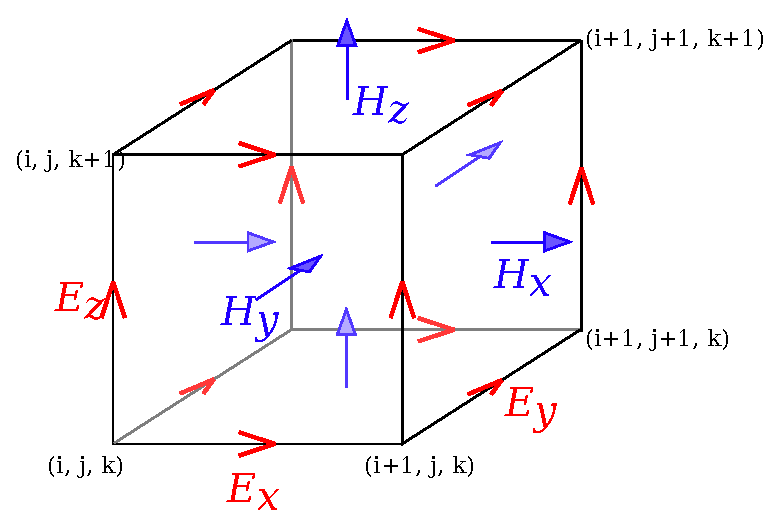
\includegraphics[width=.5\textwidth]{Yee-cube}
 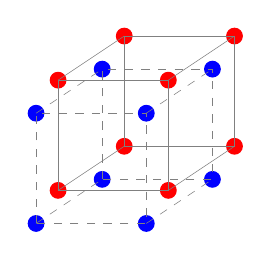
\begin{tikzpicture}[scale=.7]
    
    \foreach \x in {0,1}{
      \foreach \y in {0,1}{
        \node[mpoint] at (2*\x,2*\y) {}; 
        \node[mpoint] at (2*\x+1.2,2*\y+0.8) {}; 
        \node[epoint] at (2*\x+1.6,2*\y+1.4) {};
        \node[epoint] at (2*\x+1.6-1.2,2*\y+1.4-0.8) {};
        \draw[mgrid] (2*\x,2*\y) -- (2*\x+1.2,2*\y+0.8);
        \draw[egrid] (2*\x+1.6,2*\y+1.4) -- (2*\x+1.6-1.2,2*\y+1.4-0.8);
      }
    }
    
    \draw[mgrid] (0,0) rectangle (2,2);
    \draw[mgrid] (1.2,0.8) rectangle (3.2,2.8);
    \draw[egrid] (1.6,1.4) rectangle (3.6,3.4);
    \draw[egrid] (1.6-1.2,1.4-0.8) rectangle (3.6-1.2,3.4-0.8);

            \end{tikzpicture}
 \captionof{figure}{Left: the Yee lattice, where each component of the EM fields is defined at a different site\cite{yee-lattice}. Right: the lattice we used, where all three components of each field are known at the same site. In both cases, electric and magnetic fields are known at different times. }
\label{fig:lattice}
\end{figure}

Using the Yee lattice, the space-derivatives in eq. (\ref{eq:maxwell}) are defined exactly where they are needed for calculating the corresponding time-derivative. 
However, this benefit is only used when the dielectric tensor is diagonal. 
In a liquid crystal with spatially-dependent optical axis, this is not true, so we used a modified lattice to account for a fully-anisotropic dielectric tensor. 

\subsection{Boundary conditions}

Equations (\ref{eq:maxwell}) assume no sources inside the cell. 
This is consistent with experimental observations, where light comes from outside, passes through the sample and is then studied. 
In the numerical method, light from outside is modelled using boundary conditions. 

At other walls of the studied cell, we simulate propagation into free space using an absorbing boundary condition. 
The absorbing boundary used is the perfectly matched layer (\textsc{PML}), a non-physicial material where each component of electromagnetic fields is split into two parts. 
Each of these components observes different electric and magnetic conductivity. 

\section{Results}

\subsection{Refraction and reflection}

\subsection{Uniform layer}

A common method for observing liquid crystal and other anisotropic materials is to put a sample between crossed polarizers. 
If the sample is isotropic, no light passes through. 
However, if the material is optically anisotropic, the intensity of transmitted light depends on the orientation of the optical axis. 
If the optical axis is uniform, forming an angle $\theta$ with the transversal plane and $\beta$ with the first polarizer, it is equal to\cite{kleman}
\begin{align}
 I &= I_0 \sin^2 2\beta \sin^2 \left[ \frac{\pi d}{\lambda_0} \left( \frac{n_o n_e}{\sqrt{n_e^2 \cos^2 \theta + n_0^2 \sin^2 \theta}} - n_o \right)\right] \nonumber
\end{align}
where $n_o$ and $n_e$ are the ordinary and extraordinary refractive indices. 

The results of the simulation, compared with the theoretical prediction, are shown on Figure \ref{fig:test-uniform}. 
We can see strong agreement, confirming the correctness of the method when using an anisotropic material. 

\begin{figure}
\centering
 \resizebox{\textwidth}{!}{\input{g_test_uniform_en}}
 \captionof{figure}{Transmittance of a sample with a uniform and anisotropic dielectric tensor. }
 \label{fig:test-uniform}
\end{figure}

\subsection{Photonic band gap}



\section{Conclusions}

\bibliographystyle{zumer}
\bibliography{magisterij}

\end{multicols}

\end{document}
